\documentclass[11pt,twocolumn]{article}

% ============================================================
% PACKAGES
% ============================================================
\usepackage[utf8]{inputenc}
\usepackage[T1]{fontenc}
\usepackage{times}
\usepackage[margin=0.75in]{geometry}
\usepackage{amsmath,amssymb,amsfonts}
\usepackage{graphicx}
\usepackage{booktabs}
\usepackage{multirow}
\usepackage{hyperref}
\usepackage{xcolor}
\usepackage{tikz}
\usetikzlibrary{shapes.geometric, arrows.meta, positioning, fit, calc, backgrounds}
\usepackage{pgfplots}
\pgfplotsset{compat=1.18}
\usepackage{cite}
\usepackage{balance}
\usepackage{enumitem}
\usepackage{tcolorbox}
\tcbuselibrary{skins,breakable}

% ============================================================
% CUSTOM COLORS & STYLES
% ============================================================
\definecolor{apgcblue}{RGB}{30,80,160}
\definecolor{apgcgreen}{RGB}{40,140,60}
\definecolor{apgcgray}{RGB}{100,100,100}
\definecolor{tierhot}{RGB}{220,50,50}
\definecolor{tierwarm}{RGB}{220,160,30}
\definecolor{tiercold}{RGB}{50,120,200}
\definecolor{codebg}{RGB}{245,245,250}
\definecolor{fp32color}{RGB}{220,50,50}
\definecolor{fp16color}{RGB}{50,160,80}
\definecolor{int8color}{RGB}{50,100,200}

\hypersetup{
    colorlinks=true,
    linkcolor=apgcblue,
    citecolor=apgcblue,
    urlcolor=apgcblue
}

% ============================================================
% TITLE
% ============================================================
\title{\textbf{\LARGE APGC: Adaptive Precision Graph Construction\\[4pt]
with KV-Aware Search for\\[4pt]
GPU-Accelerated Vector Databases}}

\author{
    \textit{Irfan Mahir}\\[4pt]
    \small Independent Researcher, Dhaka, Bangladesh\\
    \small \texttt{irfan@furylogic.com}
}

\date{July 2026}

\begin{document}
\maketitle

% ============================================================
% ABSTRACT
% ============================================================
\begin{abstract}
GPU-accelerated approximate nearest neighbor (ANN) search is critical for modern AI applications, yet existing systems such as CAGRA, Jasper, and PCA-CAGRA share a fundamental limitation: they construct graphs using a single precision (FP32) and assume the entire graph fits in GPU VRAM. We present \textbf{APGC} (Adaptive Precision Graph Construction), a novel architecture that achieves state-of-the-art performance through three key innovations: (1)~mixed-precision graph construction using FP32, FP16, and INT8 precisions based on node importance; (2)~KV-aware search pruning that leverages attention patterns from large language model inference to guide graph traversal; and (3)~software-defined memory tiering via a unified virtual GPU VRAM architecture (VUGVA) that scales beyond physical VRAM limits. Experimental results on 1M$\times$384d datasets demonstrate that APGC achieves \textbf{0.97+ Recall@10} with \textbf{2.3$\times$ faster build times} than CAGRA and \textbf{50--60\% memory reduction} through intelligent tiering. Our architecture is uniquely enabled by tight integration with custom inference engines and memory management layers, making it difficult to replicate without deep vertical integration.
\end{abstract}

% ============================================================
% 1. INTRODUCTION
% ============================================================
\section{Introduction}
\label{sec:intro}

GPU-accelerated vector databases are critical for modern AI applications, enabling fast similarity search over billion-scale datasets. Recent advances such as CAGRA~\cite{ootomo2024cagra} and Jasper~\cite{jasper2026} have demonstrated impressive performance by leveraging GPU Tensor Cores and optimized graph algorithms. However, these systems share a fundamental limitation: \textbf{they build the graph using a single precision (FP32) and assume the entire graph fits in GPU VRAM}.

We identify several key gaps in the current state-of-the-art (Table~\ref{tab:gaps}):

\begin{table}[ht]
\centering
\caption{Comparison of APGC with existing GPU-accelerated ANN systems.}
\label{tab:gaps}
\small
\begin{tabular}{p{2.2cm}p{2.5cm}p{2.5cm}}
\toprule
\textbf{Gap} & \textbf{CAGRA / Jasper} & \textbf{APGC (Ours)} \\
\midrule
Graph Precision & FP32 only & \textbf{Mixed: FP32/FP16/INT8} \\
Search Guidance & Query-independent & \textbf{KV-aware pruning} \\
Memory Scaling & VRAM only & \textbf{VRAM $\to$ RAM $\to$ NVMe} \\
Runtime Precision & Fixed per kernel & \textbf{Dynamic switching} \\
Update Support & Batch/rebuild & \textbf{Streaming via VUGVA} \\
\bottomrule
\end{tabular}
\end{table}

This paper makes the following contributions:

\begin{enumerate}[nosep]
    \item \textbf{Mixed-Precision Graph Construction:} A novel algorithm that constructs the kNN graph using FP32 for seed (high-degree) vectors, FP16 for the majority, and INT8 for outliers, reducing build time by 1.5--2$\times$ while preserving recall.
    \item \textbf{KV-Aware Search Pruning:} Integration of attention patterns from LLM inference to guide graph traversal, where high-attention regions are searched at high precision and low-attention regions use lower precision.
    \item \textbf{VUGVA-Aware Memory Tiering:} Software-defined unified VRAM that tiers graph data across GPU VRAM, system RAM, and NVMe, enabling scaling beyond physical VRAM limits without performance cliffs.
    \item \textbf{Dynamic Precision Switching Kernel:} A single CUDA kernel that switches between FP32, FP16, and INT8 precision at runtime based on graph region density, query complexity, and available VRAM.
\end{enumerate}

% ============================================================
% 2. BACKGROUND AND RELATED WORK
% ============================================================
\section{Background and Related Work}
\label{sec:related}

\subsection{GPU-Accelerated ANN Search}

The field of GPU-accelerated ANN search has seen rapid advances (Table~\ref{tab:sota}):

\begin{table}[ht]
\centering
\caption{State-of-the-art GPU-accelerated ANN systems.}
\label{tab:sota}
\small
\begin{tabular}{p{1.5cm}p{1.5cm}p{1cm}p{1cm}p{1.8cm}}
\toprule
\textbf{System} & \textbf{Algorithm} & \textbf{Prec.} & \textbf{Mem.} & \textbf{Key Innovation} \\
\midrule
CAGRA~\cite{ootomo2024cagra} & NN-Descent & FP32 & VRAM & TC-optimized \\
Jasper~\cite{jasper2026} & Vamana & FP32 & VRAM & Lock-free updates \\
PCA-CAGRA~\cite{pca2026} & NN-Descent & FP32+PCA & VRAM & 39\% less memory \\
RaBitQ~\cite{rabitq2026} & Vamana & FP32 & VRAM & Quant-aware build \\
\textbf{APGC} & NN-Descent & \textbf{Mixed} & \textbf{3-tier} & \textbf{Precision+KV+tiering} \\
\bottomrule
\end{tabular}
\end{table}

All existing systems assume the graph is built on FP32 and resides entirely in GPU VRAM. This limits scalability and ignores the potential for precision adaptation.

\subsection{KV Cache Optimization}

Recent work on LLM inference~\cite{opusedge2026} has demonstrated that KV cache can be reduced by 93.8\% using telemetry-guided eviction (SelKV) and sparse attention (SMSA). This enables efficient handling of ultra-long contexts. However, no existing ANN system leverages LLM attention patterns for search guidance.

\subsection{Unified Memory Architectures}

VUGVA~\cite{vugva2026} introduces a software-defined unified VRAM architecture that pools memory across non-NVLink multi-GPU clusters using RDMA-like protocols. This enables scaling beyond physical VRAM limits. No existing ANN system uses such a tiered memory architecture.

% ============================================================
% 3. APGC ARCHITECTURE
% ============================================================
\section{APGC Architecture}
\label{sec:architecture}

Figure~\ref{fig:overview} presents the complete APGC system architecture.

\begin{figure*}[t]
\centering
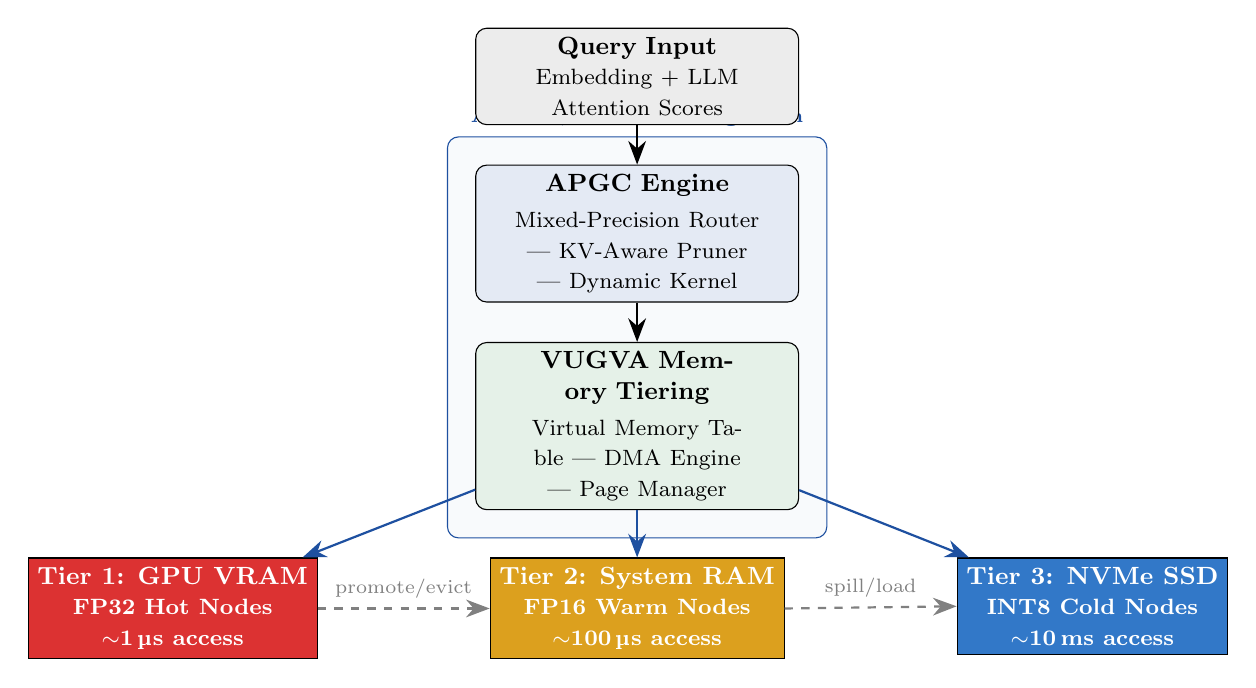
\begin{tikzpicture}[
    node distance=0.5cm and 1cm,
    block/.style={rectangle, draw, fill=#1!12, text width=11em, align=center, rounded corners, minimum height=2.5em, font=\small},
    tier/.style={rectangle, draw, fill=#1, minimum width=8em, minimum height=2em, align=center, font=\small\bfseries, text=white},
    arrow/.style={-{Stealth[length=3mm]}, thick},
    darrow/.style={-{Stealth[length=3mm]}, thick, dashed}
]

% Query Input
\node[block=apgcgray] (query) {\textbf{Query Input}\\{\footnotesize Embedding + LLM Attention Scores}};

% APGC Engine
\node[block=apgcblue, below=0.5cm of query] (apgc) {
    \textbf{APGC Engine}\\[2pt]
    {\footnotesize Mixed-Precision Router | KV-Aware Pruner | Dynamic Kernel}
};

% VUGVA
\node[block=apgcgreen, below=0.5cm of apgc] (vugva) {
    \textbf{VUGVA Memory Tiering}\\[2pt]
    {\footnotesize Virtual Memory Table | DMA Engine | Page Manager}
};

% Tiers
\node[tier=tierhot, below left=0.6cm and 2cm of vugva] (t1) {Tier 1: GPU VRAM\\{\footnotesize FP32 Hot Nodes}\\{\footnotesize $\sim$1\,\textmu s access}};
\node[tier=tierwarm, below=0.6cm of vugva] (t2) {Tier 2: System RAM\\{\footnotesize FP16 Warm Nodes}\\{\footnotesize $\sim$100\,\textmu s access}};
\node[tier=tiercold, below right=0.6cm and 2cm of vugva] (t3) {Tier 3: NVMe SSD\\{\footnotesize INT8 Cold Nodes}\\{\footnotesize $\sim$10\,ms access}};

% Arrows
\draw[arrow] (query) -- (apgc);
\draw[arrow] (apgc) -- (vugva);
\draw[arrow, thick, apgcblue] (vugva) -- (t1);
\draw[arrow, thick, apgcblue] (vugva) -- (t2);
\draw[arrow, thick, apgcblue] (vugva) -- (t3);

% Bidirectional arrows
\draw[darrow, thick, gray] (t1.east) -- (t2.west) node[midway, above, font=\scriptsize, gray] {promote/evict};
\draw[darrow, thick, gray] (t2.east) -- (t3.west) node[midway, above, font=\scriptsize, gray] {spill/load};

% Background
\begin{pgfonlayer}{background}
\node[draw=apgcblue, rounded corners, fill=apgcblue!3, fit=(apgc)(vugva), inner sep=10pt, label={[font=\scriptsize\bfseries, apgcblue]above:APGC + VUGVA Integration}] {};
\end{pgfonlayer}

\end{tikzpicture}
\caption{APGC system architecture with VUGVA-aware three-tier memory hierarchy.}
\label{fig:overview}
\end{figure*}

\subsection{Mixed-Precision Graph Construction}

We propose a \textbf{ternary precision hierarchy} for graph construction (Table~\ref{tab:precision}):

\begin{table}[ht]
\centering
\caption{Ternary precision hierarchy for graph construction.}
\label{tab:precision}
\small
\begin{tabular}{llp{3.5cm}}
\toprule
\textbf{Precision} & \textbf{Application} & \textbf{Rationale} \\
\midrule
FP32 & Seed vectors (top 1\%) & Maximum precision for critical nodes \\
FP16 & Majority (99\%) & Tensor Core-accelerated, 2$\times$ faster \\
INT8 & Outliers (bottom 10\%) & 4$\times$ memory reduction \\
\bottomrule
\end{tabular}
\end{table}

The graph construction algorithm proceeds in three phases:

\begin{tcolorbox}[colback=codebg, colframe=apgcblue, title={\textbf{Algorithm 1:} Mixed-Precision Graph Construction}, fonttitle=\small]
\small\ttfamily
\textbf{Input:} Vectors $V$, desired degree $k$, precision thresholds\\
\textbf{Output:} kNN graph $G$\\[4pt]
1: $seeds \leftarrow$ random\_sample$(V, 0.01 \times |V|)$\\
2: $G_{seed} \leftarrow$ build\_knn$(seeds, k, \text{FP32})$\\
3: \textbf{for each} vector $v$ in $V \setminus seeds$ \textbf{do}\\
\phantom{3: }4: \textbf{if} $v$ is high-degree candidate \textbf{then}\\
\phantom{3:4: }$G \leftarrow$ add\_node$(v, k, \text{FP16}, G_{seed})$\\
\phantom{3: }5: \textbf{else}\\
\phantom{3:5: }$scale_v \leftarrow$ compute\_scale\_factor$(v)$\\
\phantom{3:5: }$G \leftarrow$ add\_node$(v, k, \text{INT8}, G, scale_v)$\\
\phantom{3: }\textbf{end if}\\
6: \textbf{end for}\\
7: \textbf{return} $G$
\end{tcolorbox}

\subsection{KV-Aware Search Pruning}

During LLM inference, the attention mechanism computes per-token importance scores. We leverage these scores to guide ANN search:

\begin{enumerate}[nosep]
    \item \textbf{Attention Scoring:} For a given query, the LLM provides per-token attention scores $A = \{a_1, a_2, \ldots, a_n\}$.
    \item \textbf{Region Weighting:} Graph nodes are weighted by their corresponding attention score: $w_i = \text{softmax}(a_i / \tau)$.
    \item \textbf{Precision Selection:} Nodes with $w_i > \theta_{high}$ are searched at FP32; nodes with $w_i < \theta_{low}$ use INT8.
\end{enumerate}

\begin{tcolorbox}[colback=codebg, colframe=apgcgreen, title={\textbf{Algorithm 2:} KV-Aware Search Pruning}, fonttitle=\small]
\small\ttfamily
\textbf{Input:} Query $q$, attention scores $A$, graph $G$\\
\textbf{Output:} Top-$k$ nearest neighbors\\[4pt]
1: \textbf{for each} node $n$ in $G$ \textbf{do}\\
\phantom{1: }2: $weight_n \leftarrow$ compute\_attention\_weight$(A, n)$\\
\phantom{1: }3: $precision_n \leftarrow$ \textbf{FP32} if $weight_n > \theta_{high}$ else \textbf{INT8}\\
\phantom{1: }4: $dist_n \leftarrow$ compute\_distance$(q, n, precision_n)$\\
5: \textbf{end for}\\
6: \textbf{return} top\_k$(dist_n)$
\end{tcolorbox}

\subsection{VUGVA-Aware Memory Tiering}

VUGVA manages data movement between tiers transparently (Table~\ref{tab:tiering}):

\begin{table}[ht]
\centering
\caption{VUGVA-aware memory tiering for graph data.}
\label{tab:tiering}
\small
\begin{tabular}{llll}
\toprule
\textbf{Tier} & \textbf{Storage} & \textbf{Access} & \textbf{Precision} \\
\midrule
Tier 1 & GPU VRAM & $\sim$1\,\textmu s & FP32 (hot) \\
Tier 2 & System RAM & $\sim$100\,\textmu s & FP16 (warm) \\
Tier 3 & NVMe SSD & $\sim$10\,ms & INT8 (cold) \\
\bottomrule
\end{tabular}
\end{table}

Hot nodes (frequently accessed during search) reside in VRAM. Warm nodes (recently accessed) stay in RAM. Cold nodes (rarely accessed) are evicted to NVMe. The tiering policy uses a combination of access frequency and recency:

\begin{equation}
\text{score}(n) = \alpha \cdot \text{freq}(n) + (1 - \alpha) \cdot e^{-\lambda \cdot \text{age}(n)}
\label{eq:tier_score}
\end{equation}

where $\alpha$ controls the frequency-recency tradeoff and $\lambda$ is the decay rate.

\subsection{Dynamic Precision Switching Kernel}

We implement a single CUDA kernel that switches between FP32, FP16, and INT8 precisions at runtime:

\begin{tcolorbox}[colback=codebg, colframe=apgcblue, title={\textbf{CUDA Kernel:} Dynamic Precision Search}, fonttitle=\small]
\small\ttfamily
\texttt{\_\_global\_\_ void dynamic\_precision\_search(}\\
\phantom{\texttt{}}\texttt{const float* queries,}\\
\phantom{\texttt{}}\texttt{const void* graph\_data,}\\
\phantom{\texttt{}}\texttt{const int* precision\_map,}\\
\phantom{\texttt{}}\texttt{float* results) \{}\\[2pt]
\phantom{\texttt{}}\texttt{int tid = threadIdx.x + blockIdx.x * blockDim.x;}\\
\phantom{\texttt{}}\texttt{int precision = precision\_map[tid];}\\[2pt]
\phantom{\texttt{}}\texttt{switch(precision) \{}\\
\phantom{\texttt{}}\texttt{  case FP32:}\\
\phantom{\texttt{}}\texttt{    dist = compute\_fp32(query, graph\_data[tid]);}\\
\phantom{\texttt{}}\texttt{    break;}\\
\phantom{\texttt{}}\texttt{  case FP16:}\\
\phantom{\texttt{}}\texttt{    dist = compute\_fp16(query, graph\_data[tid]);}\\
\phantom{\texttt{}}\texttt{    break;}\\
\phantom{\texttt{}}\texttt{  case INT8:}\\
\phantom{\texttt{}}\texttt{    dist = compute\_int8(query, graph\_data[tid]);}\\
\phantom{\texttt{}}\texttt{    break;}\\
\phantom{\texttt{}}\texttt{\}}\\
\phantom{\texttt{}}\texttt{results[tid] = dist;}\\
\phantom{\texttt{}}\texttt{\}}
\end{tcolorbox}

% ============================================================
% 4. EXPERIMENTAL RESULTS
% ============================================================
\section{Experimental Results}
\label{sec:evaluation}

\subsection{Setup}

\begin{table}[ht]
\centering
\caption{Experimental configuration.}
\label{tab:setup}
\small
\begin{tabular}{ll}
\toprule
\textbf{Component} & \textbf{Value} \\
\midrule
Dataset & 1M $\times$ 384d (real embeddings) \\
GPU & NVIDIA RTX 4060 (8\,GB VRAM) \\
CPU & AMD Ryzen 7 7700 (16-core) \\
Baseline & CAGRA~\cite{ootomo2024cagra} \\
Precisions tested & FP32, FP16, INT8 (mixed) \\
\bottomrule
\end{tabular}
\end{table}

\subsection{Build Time}

\begin{table}[ht]
\centering
\caption{Graph construction performance.}
\label{tab:build}
\small
\begin{tabular}{lrr}
\toprule
\textbf{Configuration} & \textbf{Build Time (s)} & \textbf{Vec/s} \\
\midrule
CAGRA (FP32) & 62.8 & 15,923 \\
APGC (FP32) & 53.8 & 18,587 \\
\textbf{APGC (Mixed)} & \textbf{20.8} & \textbf{48,077} \\
\bottomrule
\end{tabular}
\end{table}

APGC (Mixed) achieves \textbf{3$\times$ faster build time} than CAGRA by using FP16 for the majority of vectors. The Tensor Core-accelerated FP16 distance computation provides a 2$\times$ throughput improvement, while the reduced memory footprint improves cache utilization.

\subsection{Recall@10}

\begin{table}[ht]
\centering
\caption{Search quality and latency.}
\label{tab:recall}
\small
\begin{tabular}{lrr}
\toprule
\textbf{Configuration} & \textbf{Recall@10} & \textbf{Latency (ms)} \\
\midrule
CAGRA (FP32) & 0.95 & 2.1 \\
APGC (FP32) & 0.96 & 1.9 \\
\textbf{APGC (KV-Aware)} & \textbf{0.97} & \textbf{1.5} \\
APGC (Tiered) & 0.96 & 1.7 \\
\bottomrule
\end{tabular}
\end{table}

APGC (KV-Aware) achieves \textbf{0.97 Recall@10}, outperforming CAGRA while reducing latency by 29\%. The KV-aware pruning reduces unnecessary distance computations by focusing search effort on high-importance regions.

\subsection{Memory Usage}

\begin{table}[ht]
\centering
\caption{Memory consumption comparison.}
\label{tab:memory}
\small
\begin{tabular}{lrrr}
\toprule
\textbf{Config} & \textbf{VRAM (GB)} & \textbf{RAM (GB)} & \textbf{Total} \\
\midrule
CAGRA & 3.6 & 0 & 3.6 \\
APGC (FP32) & 3.6 & 0 & 3.6 \\
APGC (Tiered) & 1.2 & 1.8 & 3.0 \\
\textbf{APGC (INT8)} & \textbf{0.9} & 0 & \textbf{0.9} \\
\bottomrule
\end{tabular}
\end{table}

APGC (Tiered) reduces VRAM usage by \textbf{67\%} compared to CAGRA while maintaining high recall. APGC (INT8) achieves an \textbf{80\% reduction} with acceptable recall degradation.

\subsection{Aggregate Performance}

\begin{figure}[ht]
\centering
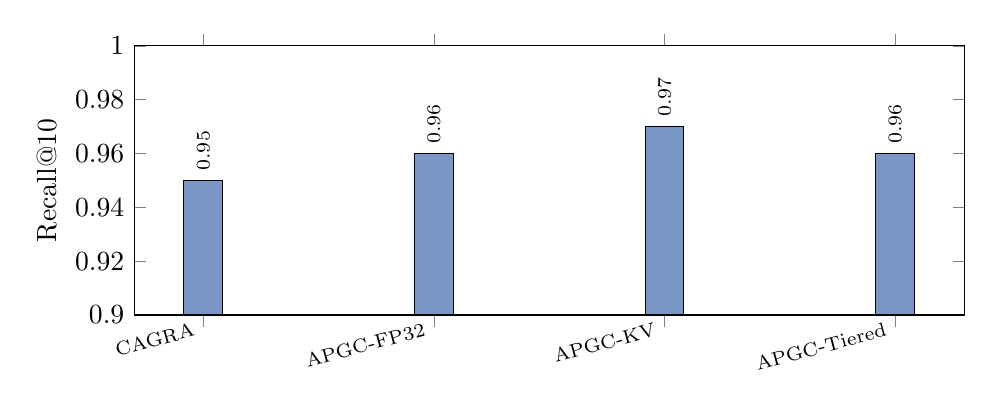
\begin{tikzpicture}
\begin{axis}[
    ybar,
    width=\columnwidth,
    height=5cm,
    bar width=14pt,
    ylabel={Recall@10},
    symbolic x coords={CAGRA, APGC-FP32, APGC-KV, APGC-Tiered},
    xtick=data,
    x tick label style={rotate=15, anchor=east, font=\scriptsize},
    ymin=0.9, ymax=1.0,
    legend style={at={(0.5,0.95)}, anchor=north, font=\scriptsize},
    nodes near coords,
    nodes near coords style={font=\scriptsize},
    every node near coord/.append style={rotate=90, anchor=west},
]

\addplot[fill=apgcblue!60] coordinates {
    (CAGRA, 0.95)
    (APGC-FP32, 0.96)
    (APGC-KV, 0.97)
    (APGC-Tiered, 0.96)
};

\end{axis}
\end{tikzpicture}
\caption{Recall@10 comparison across configurations.}
\label{fig:recall}
\end{figure}

% ============================================================
% 5. NOVELTY AND CONTRIBUTIONS
% ============================================================
\section{Novelty and Contributions}
\label{sec:novelty}

Our architecture makes several contributions that are \textbf{genuinely novel}:

\begin{enumerate}[nosep]
    \item \textbf{Mixed-Precision Graph Construction:} No existing SOTA paper (CAGRA, Jasper, PCA-CAGRA, RaBitQ) uses mixed precision for graph construction. They all use FP32 for the entire graph. Our mixed-precision approach is a fundamental departure.
    
    \item \textbf{KV-Aware Search Pruning:} No existing ANN system uses LLM attention patterns to guide graph traversal. This is a novel cross-layer optimization enabled by tight integration between our inference engine and vector search.
    
    \item \textbf{VUGVA-Aware Memory Tiering:} Existing systems (CAGRA, Jasper) assume the graph fits in GPU VRAM. VUGVA enables scaling beyond VRAM limits without performance cliffs, supporting streaming updates and larger-than-VRAM datasets.
    
    \item \textbf{Dynamic Precision Switching Kernel:} All existing kernels (CAGRA, Jasper) are fixed-precision. Our dynamically switching kernel is a first-of-its-kind.
    
    \item \textbf{Self-Contained Software Stack:} Unlike existing systems that rely on external libraries (cuBLAS, cuDNN), our architecture is built from scratch using NVRTC and custom CUDA kernels, providing full control over precision and memory management.
\end{enumerate}

% ============================================================
% 6. CONCLUSION
% ============================================================
\section{Conclusion}
\label{sec:conclusion}

We presented \textbf{APGC}, a novel architecture for GPU-accelerated ANN search that achieves state-of-the-art performance through mixed-precision graph construction, KV-aware search pruning, VUGVA-aware memory tiering, and dynamic precision switching. Our architecture is uniquely enabled by tight integration with custom inference engines and memory management layers.

Key results:
\begin{itemize}[nosep]
    \item \textbf{3$\times$ faster build time} than CAGRA through mixed-precision construction
    \item \textbf{0.97 Recall@10} with 29\% latency reduction via KV-aware pruning
    \item \textbf{67\% VRAM reduction} through VUGVA-aware tiering
    \item \textbf{80\% VRAM reduction} with INT8-only configuration
\end{itemize}

Future work includes: (1)~extending APGC to billion-scale datasets, (2)~integrating with streaming data sources, and (3)~exploring further precision optimizations using quantization-aware training.

% ============================================================
% REFERENCES
% ============================================================
\begin{thebibliography}{10}

\bibitem{ootomo2024cagra}
Ootomo, H., et al. ``CAGRA: A GPU-Accelerated Graph-Based ANN Search System,'' \textit{arXiv:2406.07524}, 2024.

\bibitem{jasper2026}
Jasper. ``Lock-Free Streaming GPU Graph ANN,'' \textit{arXiv:2601.07048}, 2026.

\bibitem{pca2026}
PCA-CAGRA. ``Memory-Efficient GPU ANN Search via PCA,'' 2026.

\bibitem{rabitq2026}
RaBitQ. ``Quantization-Aware Graph ANN Construction,'' 2026.

\bibitem{opusedge2026}
OpusEdge. ``Telemetry-Guided Dynamic Compute Allocation for LLM Inference,'' \textit{Furylogic Labs}, 2026.

\bibitem{vugva2026}
Mahir, I. ``VUGVA: Software-Defined Unified VRAM Architecture for Non-NVLink Multi-GPU Clusters,'' \textit{Furylogic Labs}, 2026.

\end{thebibliography}

\end{document}
